\documentclass[12pt, letterpaper]{article}
\usepackage[utf8]{inputenc}
\usepackage{graphicx}  % Required for inserting images
\usepackage{amssymb}
\usepackage{amsmath}
\usepackage{enumitem}
\usepackage{fancyhdr}
\usepackage{geometry}

\graphicspath{ {./images/} }
\geometry{margin = 1in}
\renewcommand{\arraystretch}{1.5}
\linespread{2}

% Macros
\newcommand{\onespace}{\hspace*{1ex}}
\newcommand{\skipline}{\\[2\baselineskip]}
\newcommand{\tab}{\hspace*{4ex}}

\title{ECS 132 Term Project}
\author{\\ Ethan Wang}
\date{}
\pagestyle{fancy}
\setlength{\headheight}{41.68335pt}
\setlength\parindent{14pt}

\begin{document}

\maketitle

% Exponential Family
\newpage
\noindent
\section*{Exponential Distribution}
\normalsize
Initial Density Estimates\\
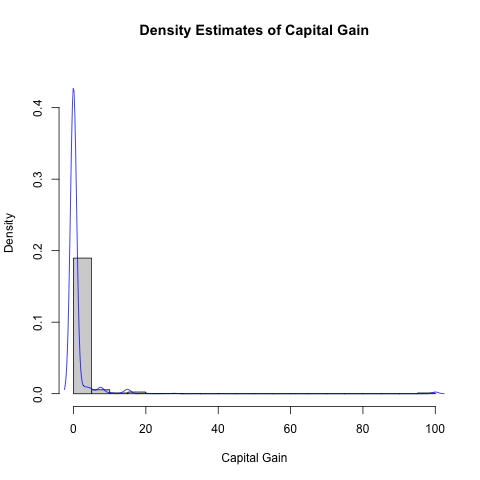
\includegraphics[scale=0.9]{capital_gain_density_estimates}
\newpage
\noindent
Using method of moments to estimate $\lambda$
\begin{flalign*}
    E(X) &= \frac{1}{\lambda}, L = \lambda\\
    \overline{A} &= \frac{1}{L}\\
    L &= \frac{\ 1\ }{\overline{A}}\\
    &\approx 0.916
\end{flalign*}
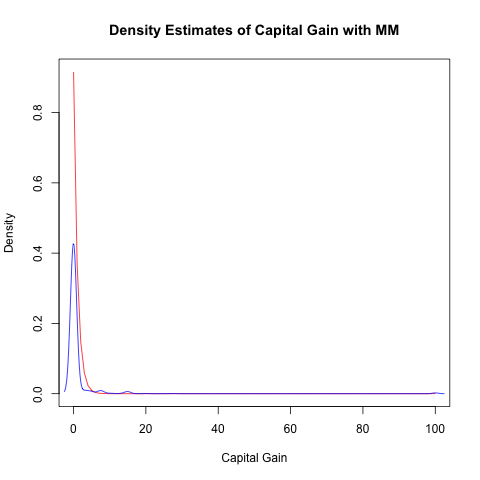
\includegraphics[scale=0.9]{capital_gain_mm}
\footnotesize
\\ \**The blue curve is the plot of density(), the red curve uses the estimated $\lambda$ in a plot of dexp()
\newpage
\noindent
\normalsize
Using method of maximum likelihood to estimate $\lambda$\\
Log Likelihood Expression Derivation
\begin{flalign*}
    \prod^{n}_{i = 1} {\lambda}e^{-{\lambda}X_i} &= {\lambda}^ne^{-{\lambda}\sum^{n}_{i=1}X_i}
    \\[1\baselineskip]
    \ln(\frac{\lambda^n}{e^{{\lambda}\sum^{n}_{i=1}X_i}}) &= \ln(\lambda^n) - \ln(e^{{\lambda}\sum^{n}_{i=1}X_i})\\
    &= n\ln(\lambda) - {\lambda}\sum^{n}_{i=1}X_i
    \\[1\baselineskip]
    \text{MLE estimated } \lambda &\approx 0.916
\end{flalign*}
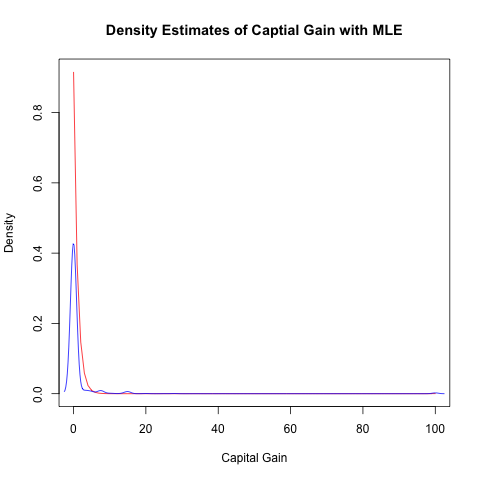
\includegraphics[scale=0.9]{capital_gain_mle}
\footnotesize
\\ \**The blue curve is the plot of density(), the red curve uses the estimated $\lambda$ in a plot of dexp()
\newpage
\noindent
\normalsize
In Professor Matloff's fastStat lesson, ``MLEMM: General Methods of Estimation," both the method of 
moments estimator and the maximum likelihood estimator for the parameter $\lambda$ of an exponential 
distribution was $\frac{\ 1\ }{\overline{A}}$. However, the mle function from the stats4 
library was used to estimate $\lambda$ instead of using $\frac{\ 1\ }{\overline{A}}$ directly for the 
maximum likelihood estimator, both for consistency across our work and as an extra verification measure. 
As expected, both estimators yielded a result of about 0.916. The graph of the exponential distribution 
PDF using the estimated $\lambda$ closely follows that of the density curve of the data, which suggests 
that an exponential distribution is a suitable approximation for the population density of this dataset.


% Gamma Family
\newpage
\noindent
\section*{Gamma Distribution}
\normalsize
Initial Density Estimates\\
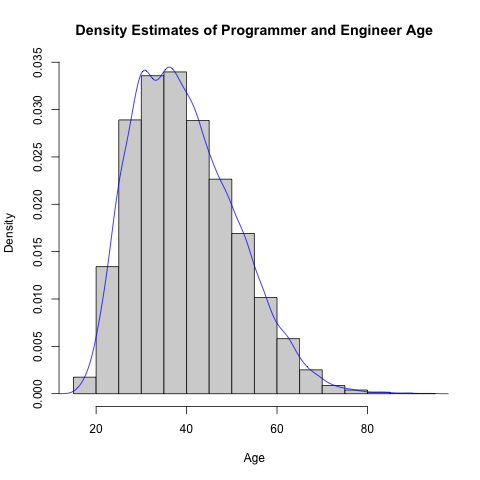
\includegraphics[scale=0.9]{prgeng_age_density_estimates}
\newpage
\noindent
Using method of moments to estimate $\lambda$ and $r$
\begin{flalign*}
    E(X) &= \frac{r}{\lambda}, L = \lambda, R = r\\
    \sigma^2 &= \frac{r}{\lambda^2}\\
    \overline{A} &= \frac{R}{L}\\
    S^2 &= \frac{R}{L^2}\\
    \\[1\baselineskip]
    R &= L\overline{A}\\
    S^2 &= \frac{L\overline{A}}{L^2}\\
    &= \frac{\overline{A}}{L}\\
    L &= \frac{\overline{A}}{S^2}\\
    &\approx 0.314\\
    R &\approx 12.421
\end{flalign*}
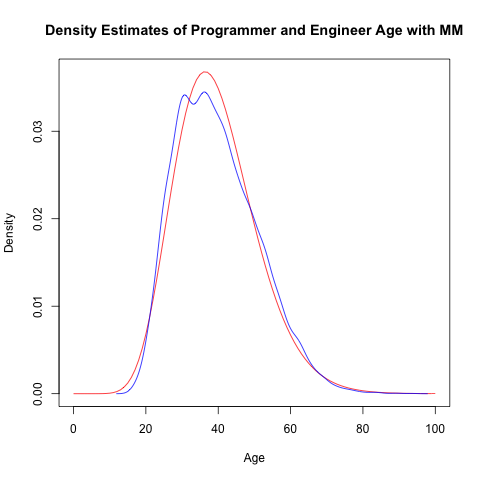
\includegraphics[scale=0.9]{prgeng_age_mm}
\footnotesize
\\ \**The blue curve is the plot of density(), the red curve uses the estimated {$\lambda$} and $r$ in a plot of dgamma()
\newpage
\noindent
\normalsize
Using method of maximum likelihood to estimate $\lambda$ and r\\
Log Likelihood Expression Derivation
\begin{flalign*}
    \prod^{n}_{i = 1} \frac{{\lambda}^rX_i^{r-1}}{\Gamma(r)e^{{\lambda}X_i}} &= (\frac{\lambda^r}{\Gamma(r)})^n \ast \prod^n_{i=1}X_i^{r-1} \ast \frac{1}{e^{{\lambda}\sum^n_{i=1}X_i}}
    \\[1\baselineskip]
    \ln((\frac{\lambda^r}{\Gamma(r)})^n \ast \prod^n_{i=1}X_i^{r-1} \ast \frac{1}{e^{{\lambda}\sum^n_{i=1}X_i}}) &= \ln(\lambda^{rn}) + \ln(\prod^n_{i=1}X_i^{r-1}) - \ln(e^{{\lambda}\sum^{n}_{i=1}X_i}) - \ln((\Gamma(r))^n)\\
    &= rn\ln(\lambda) + (r-1)\sum^n_{i=1}\ln(X_i) - {\lambda}\sum^{n}_{i=1}X_i - n\ln(\Gamma(r))
    \\[1\baselineskip]
    \text{MLE estimated } \lambda &\approx 0.320\\
    \text{MLE estimated } r &\approx 12.643
\end{flalign*}
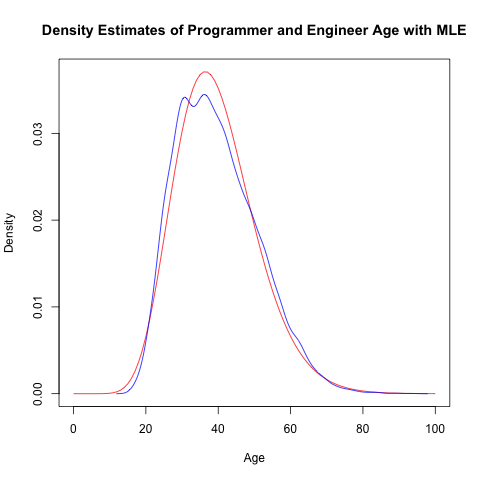
\includegraphics[scale=0.9]{prgeng_age_mle}
\footnotesize
\\ \**The blue curve is the plot of density(), the red curve uses the estimated {$\lambda$} and $r$ in a plot of dgamma()
\newpage
\noindent
\normalsize
For the data chosen to be approximated by a gamma distribution, the estimated values for $\lambda$ and $r$ 
have little difference from one method of forming estimators to the other. The graphs of the gamma 
distribution PDF using the estimated $\lambda$ and $r$ parameters for each estimation fit the density 
curve of the data well, suggesting that a gamma distribution is a suitable approximation for the 
population density of this dataset. One concern is that the peaks of both PDFs are slightly to the right 
of the one in the original density graph, although it is not by much.


% Contribution Section
\newpage
\begin{center}
    \section*{Team Member Contributions}
\end{center}

\normalsize
Ethan Wang
\begin{itemize}[leftmargin=50pt]
  \item Exponential and gamma distributions (data and analysis)
  \item R code in exp\_and\_gamma.R
\end{itemize}


\end{document}

